\begin{exercise}

Bestimmen und skizzieren Sie diejenigen Gebiete in $\R^2$, fur welche die folgenden Differentialgleichungen jeweils elliptisch, parabolisch oder hyperbolisch sind:

\begin{enumerate}[label = (\roman*)]
    \item $(y^2 + 1) u_{xx} + 2 x u_{xy} + 9 u_{yy} - u u_y = y^2 - x$,
    \item $x u_{xx} + 2 y u_{xy} + u_{yy} + x u_x = 1$.
\end{enumerate}

\end{exercise}

\begin{solution}
	\begin{figure}[h!]
		\centering
		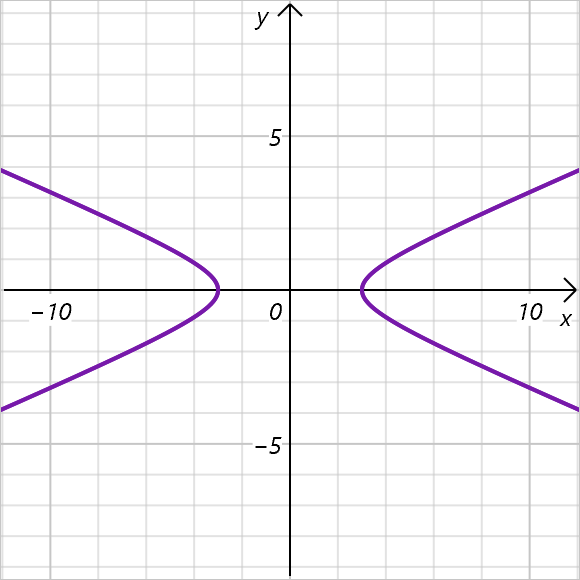
\includegraphics{../2.1.1.png}
		\caption{$x = \pm 3 \sqrt{y^2 + 1}$}
		\label{fig:(i)}
	\end{figure}
	\begin{figure}[h!]
		\centering
		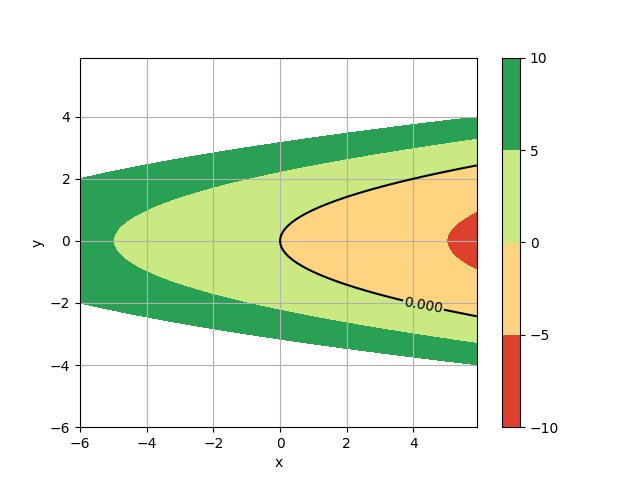
\includegraphics{../2.1.2.png}
		\caption{$x = y^2$}
		\label{fig:(ii)}
	\end{figure}
	\begin{enumerate}[label = (\roman*)]
		\item Wir definieren 
		\begin{align*}
			a(x,y) := (y^2 + 1), \qquad b(x,y) := x, \qquad c(x,y) := 9 
		\end{align*}
		und erhalten nach Definiton, dass wir es mit einer parabolischen Gleichung zu tun haben, falls $\left(b(x,y)\right)^2 - a(x,y)c(x,y) = 0$ ist. Setzen wir ein so erhalten wir die Gleichung
		\begin{align*}
		x^2 = 9(1 + y^2) \Leftrightarrow x = \pm 3\sqrt{1 + y^2},
		\end{align*}
		deren Lösungsmenge wir in Abbildung \ref{fig:(i)} sehen. Bereits aus der Gleichung erkennt man die Spiegelsymmetrie an den beiden Achsen. Die Kurve teilt den $\R^2$ in drei Zusammenhangskomponenten. Auf der null enthaltenden Zusammenhangskomponente ist die Gleichung elliptisch, also $\left(b(x,y)\right)^2 - a(x,y)c(x,y) < 0$ überall sonst ist sie hyperbolisch, also $\left(b(x,y)\right)^2 - a(x,y)c(x,y) > 0$.
		
		\item Nun haben wir
		\begin{align*}
		a(x,y) := x, \qquad b(x,y) := y, \qquad c(x,y) := 1 .
		\end{align*}
		Damit ist unsere Gleichung parabolisch falls
		\begin{align*}
		0 = \left(b(x,y)\right)^2 - a(x,y)c(x,y) = y^2 - x \Leftrightarrow x = y^2
		\end{align*}
		erfüllt ist. In Abbildung \ref{fig:(ii)} sehen wir wie die Lösungsmenge dieser Gleichung ausschaut. Diesmal wird der $\R^2$ nur in zwei Zusammenhangskomponenten geteilt. Auf der $(1,0)$ enthaltenden Zusammenhangskomponente ist die Gleichung elliptisch, überall sonst ist sie hyperbolisch.
	\end{enumerate}
\end{solution}

